\DiaryEntry{Primes, Distribution and Goldbach Conjecture}{2020-11-13}{Number Theory}

Although there is an infinitude of primes, their distribution within the positive integers is most mystifying. The difference between consecutive primes can be small, as with the pairs $11$ and $13$, $17$ and $19$, or for that matter $1000000000061$ and $1000000000063$. At the same time there exist arbitrarily long intervals in the sequence of integers that are totally devoid of any primes.

It is an open question whether there are any \emph{twin primes}; i.e. pairs of successive odd integers $p$ and $p+2$ that are both primes. So far, numerical evidence indicates that twin primes become very scarce for large numbers.

The largest twins to date (2009), are each $100355$ digits long and are given by

\bee
65516468355 \cdot 2^{333333} \pm 1 .
\eee

Consecutive can also be far apart with arbitrarily large gaps between primes. Givena positive integer $n$, we can construct a series of $n$ consecutive integers which are also composite. To this end, consider the length$-$ sequence

\bee
(n+1)! + 2, (n+1)! + 3, (n+1)! + 4, \ldots, (n+1)! + (n+1)
\eee

Each integer is composite; the first one is divisible by two as $\frac{1 \cdot 2 \cdot 3 \cdots (n+1) + 2}{2} = 1 \cdot 3 \cdots (n+1) + 1$, the second one is divisible by three, and so on.

As an example, we want three consecutive composite integers. We start with $(n+1)! + 2 = 4! + 2 = 24+2 = 26$ and continue as $4! + 3 = 27, 4! + 4 = 28$. However, smaller integers exist as well; e.g. $8, 9, 10$, or $14, 15, 16$.

The example suggest thatabove procedure yields too large numbers. For instance, the first prime gap of size larger than $14$ occurs between the primes $523$ and $541$, while $15!$ is the vastly larger number $1307674368000$. 

The \href{https://en.wikipedia.org/wiki/Prime_gap}{Wikpedia article} is quite comprehensive; The $n$-th prime gap $g_n$ is defined difference between the $n+1$-th and $n$-th prime; i.e.

\bee
g_n = p_{n+1} - p_n
\eee

The first values for $g_n$ are $3-2 = \mathbf{1}, 5 - 3 = \mathbf{2}, 7 - 5 = \mathbf{2}, 11 - 7 = \mathbf{4}, 13 - 11 = \mathbf{2}, 17 - 13 = \mathbf{4}, \ldots$. The OEIS is \href{https://oeis.org/A001223}{OEIS:A001223}.

A histogram of the prime gaps $g_n$ for primes below $100.000$ is shown in the following Figure. First observation is that the prime gap is always an even number (primes are odd and adding an odd gap yields an even number which cannot be prime). Prime gaps of size $6$ seem to be very common; gaps beyonf $40$ are increasingly rare.

\begin{figure}[H]
    \centering
    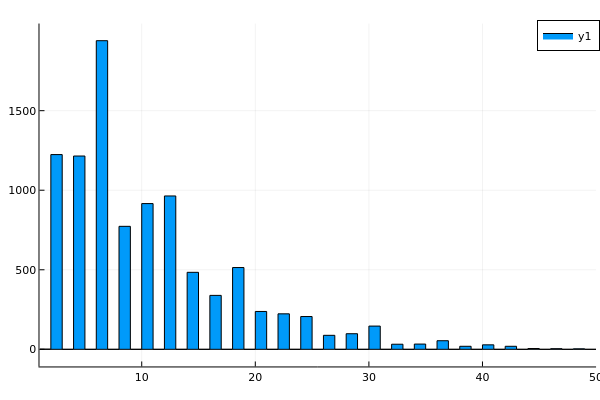
\includegraphics[scale=0.55]{images/primes_02_01.png}
\end{figure}

The \emph{Goldback Conjecture} states that every even integer is the sum of two numbers that are either primes or $1$. A somewhat more general formulation is that every even integer greater than $4$ can be written as a sum of two odd prime numbers. The numerical evidence of correctness are overwhelming, but no proof has been foumd.

%%% Local Variables:
%%% mode: latex
%%% TeX-master: "journal"
%%% End:
